\subsection{CU 11 Registrar Empleado}
En la siguiente ventana, figura \ref{fig:Pantalla Registrar Empleado - Vista de Escenarios}, se muestra un formulario de registro para un nuevo empleado donde el administrador podrá ingresar la información que el sistema le solicita para llevar a cabo el registro. Los datos que pide son: número de empleado (este será el usuario de cuenta del empleado), nombre completo y una contraseña que se le proporcionará al empleado una vez que el registro se haya hecho. En la parte inferior de la ventana, tenemos dos botones:
\begin{itemize}
	\item \textbf{Registrar:} Una vez llenados los campos, al dar click en este botón el sistema los validará y verificará si todos están llenos y con el formato adecuado, de no ser así se mostrará un mensaje de error (figura \ref{fig:Alerta Registro Empleados - Vista de Escenarios}) y el administrador debe de corregir el error de captura.
	\item \textbf{Cancelar: } El administrador desea salir de esa ventana, y el sistema regresa al a ventana 'Visualizar Empleados' (figura \ref{fig:Pantalla Visualizar Empleados - Vista de Escenarios}).
\end{itemize}
\begin{figure}[!h]
	\centering
	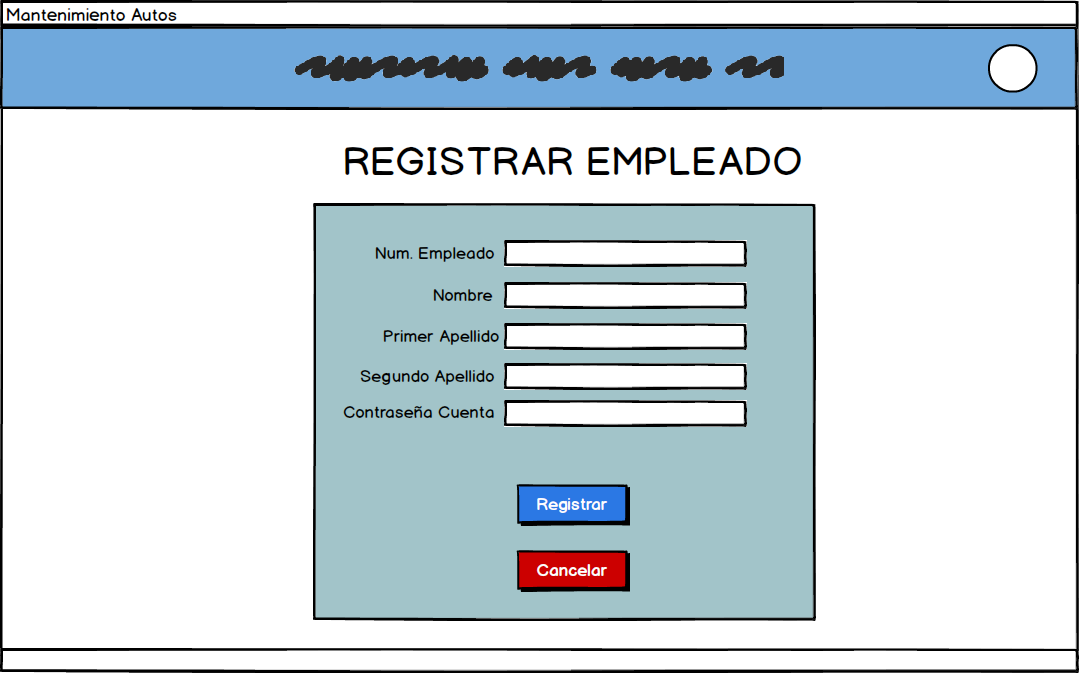
\includegraphics[width=0.8\textwidth]{./diseno/vescenarios/imagenes/registrarEmpleado}
	\caption{Pantalla Registrar Empleado - Vista de Escenarios}
	\label{fig:Pantalla Registrar Empleado - Vista de Escenarios}
\end{figure}
\begin{figure}[!h]
	\centering
	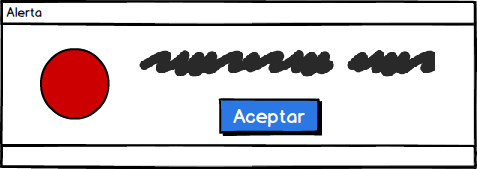
\includegraphics[width=0.3\textwidth]{./diseno/vescenarios/imagenes/alerta}
	\caption{Alerta Registro Empleados - Vista de Escenarios}
	\label{fig:Alerta Registro Empleados - Vista de Escenarios}
\end{figure}
\clearpage